\chapter{The FLRW Cosmology Universe Model}

\section{Domain}
Cosmology / General Relativistic Universe Dynamics

\section{System Model}
The Friedmann-Lemaître-Robertson-Walker (FLRW) Cosmological System (SDCM Linearized Formulation)

\section{Description}
A cosmological model of an expanding, homogeneous, and isotropic universe derived from Einstein's field equations of general relativity, governing the evolution of the cosmic scale factor under radiation, matter, and dark energy components.

\section{Set of Equations}
The governing non-linear Friedmann acceleration and fluid equations recast into State-Dependent Coefficient (SDC) matrix form $\dot{\mathbf{x}} = \mathbf{A}(\mathbf{x})\mathbf{x}$:
\begin{align}
\frac{da}{dt} &= H a \\
\frac{dH}{dt} &= -\frac{3}{2} H^2 - \frac{4\pi G}{3} (\rho_m + 3p_m) + \frac{\Lambda c^2}{3}
\end{align}
Expressed in matrix form:
\begin{equation}
\begin{pmatrix} \dot{a} \\ \dot{H} \end{pmatrix} = \begin{pmatrix} 0 & a \\ 0 & -\frac{3}{2}H - \frac{4\pi G(\rho_m + 3p_m)}{3H} + \frac{\Lambda c^2}{3H} \end{pmatrix} \begin{pmatrix} a \\ H \end{pmatrix}
\end{equation}

\section{Explanation of Terms}
\begin{itemize}
    \item $a$: Cosmological scale factor representing the relative expansion of space.
    \item $H$: Hubble parameter ($\frac{\dot{a}}{a}$), quantifying the expansion rate of the universe.
    \item $\rho_m, p_m$: Cosmic matter density and pressure.
    \item $\Lambda$: Cosmological constant representing dark energy density.
    \item $G, c$: Universal gravitational constant and speed of light.
\end{itemize}

\section{Note on the Problem}
\begin{itemize}
    \item \textbf{Context \& History:} Developed independently by Alexander Friedmann (1922) and Georges Lemaître (1927), later expanded by Howard Robertson and Arthur Walker.
    \item \textbf{Why Intractable:} The non-linear interplay between matter density dilution ($a^{-3}$), radiation scaling ($a^{-4}$), and dark energy acceleration prevents elementary closed-form analytical solutions across all cosmic epochs.
    \item \textbf{How We Solved It:} Embedding scale-dependent density transitions into the SDC matrix allows stable numerical integration of cosmic expansion curves from early deceleration to modern dark-energy-dominated acceleration.
    \item \textbf{Properties of the Solution:} Monotonic expansion of the scale factor, transition from matter-domination deceleration to cosmic acceleration, and asymptotic de Sitter exponential growth.
    \item \textbf{Prize / Significance:} The foundational framework of modern physical cosmology and observational astronomy (Nobel Prize in Physics for discovering accelerating expansion).
\end{itemize}

\section{config.py Values}
\begin{verbatim}
OMEGA_M0 = 0.315
OMEGA_L0 = 0.685
H0 = 67.4
DT = 1.0e11
TIME_STEPS = 3000
INITIAL_STATE = [0.01, 2.5e-17]
\end{verbatim}

\section{input\_data.csv Values}
\begin{verbatim}
step,t_sec,scale_factor_a,hubble_parameter_H
0,0.00,0.010,2.50e-17
1,1.0e11,0.01002,2.49e-17
...
3000,3.0e14,1.000,2.18e-18
\end{verbatim}

\section{Initial State Vector}
\begin{equation}
\mathbf{x}_0 = \begin{bmatrix} 0.01 \\ 2.5 \times 10^{-17} \end{bmatrix}
\end{equation}

\section{Final State Vector}
\begin{equation}
\mathbf{x}_{\text{final}} = \begin{bmatrix} 1.000 \\ 2.18 \times 10^{-18} \end{bmatrix}
\end{equation}



\clearpage
\section{3D Phase Plot}
\begin{figure}[h]
    \centering
    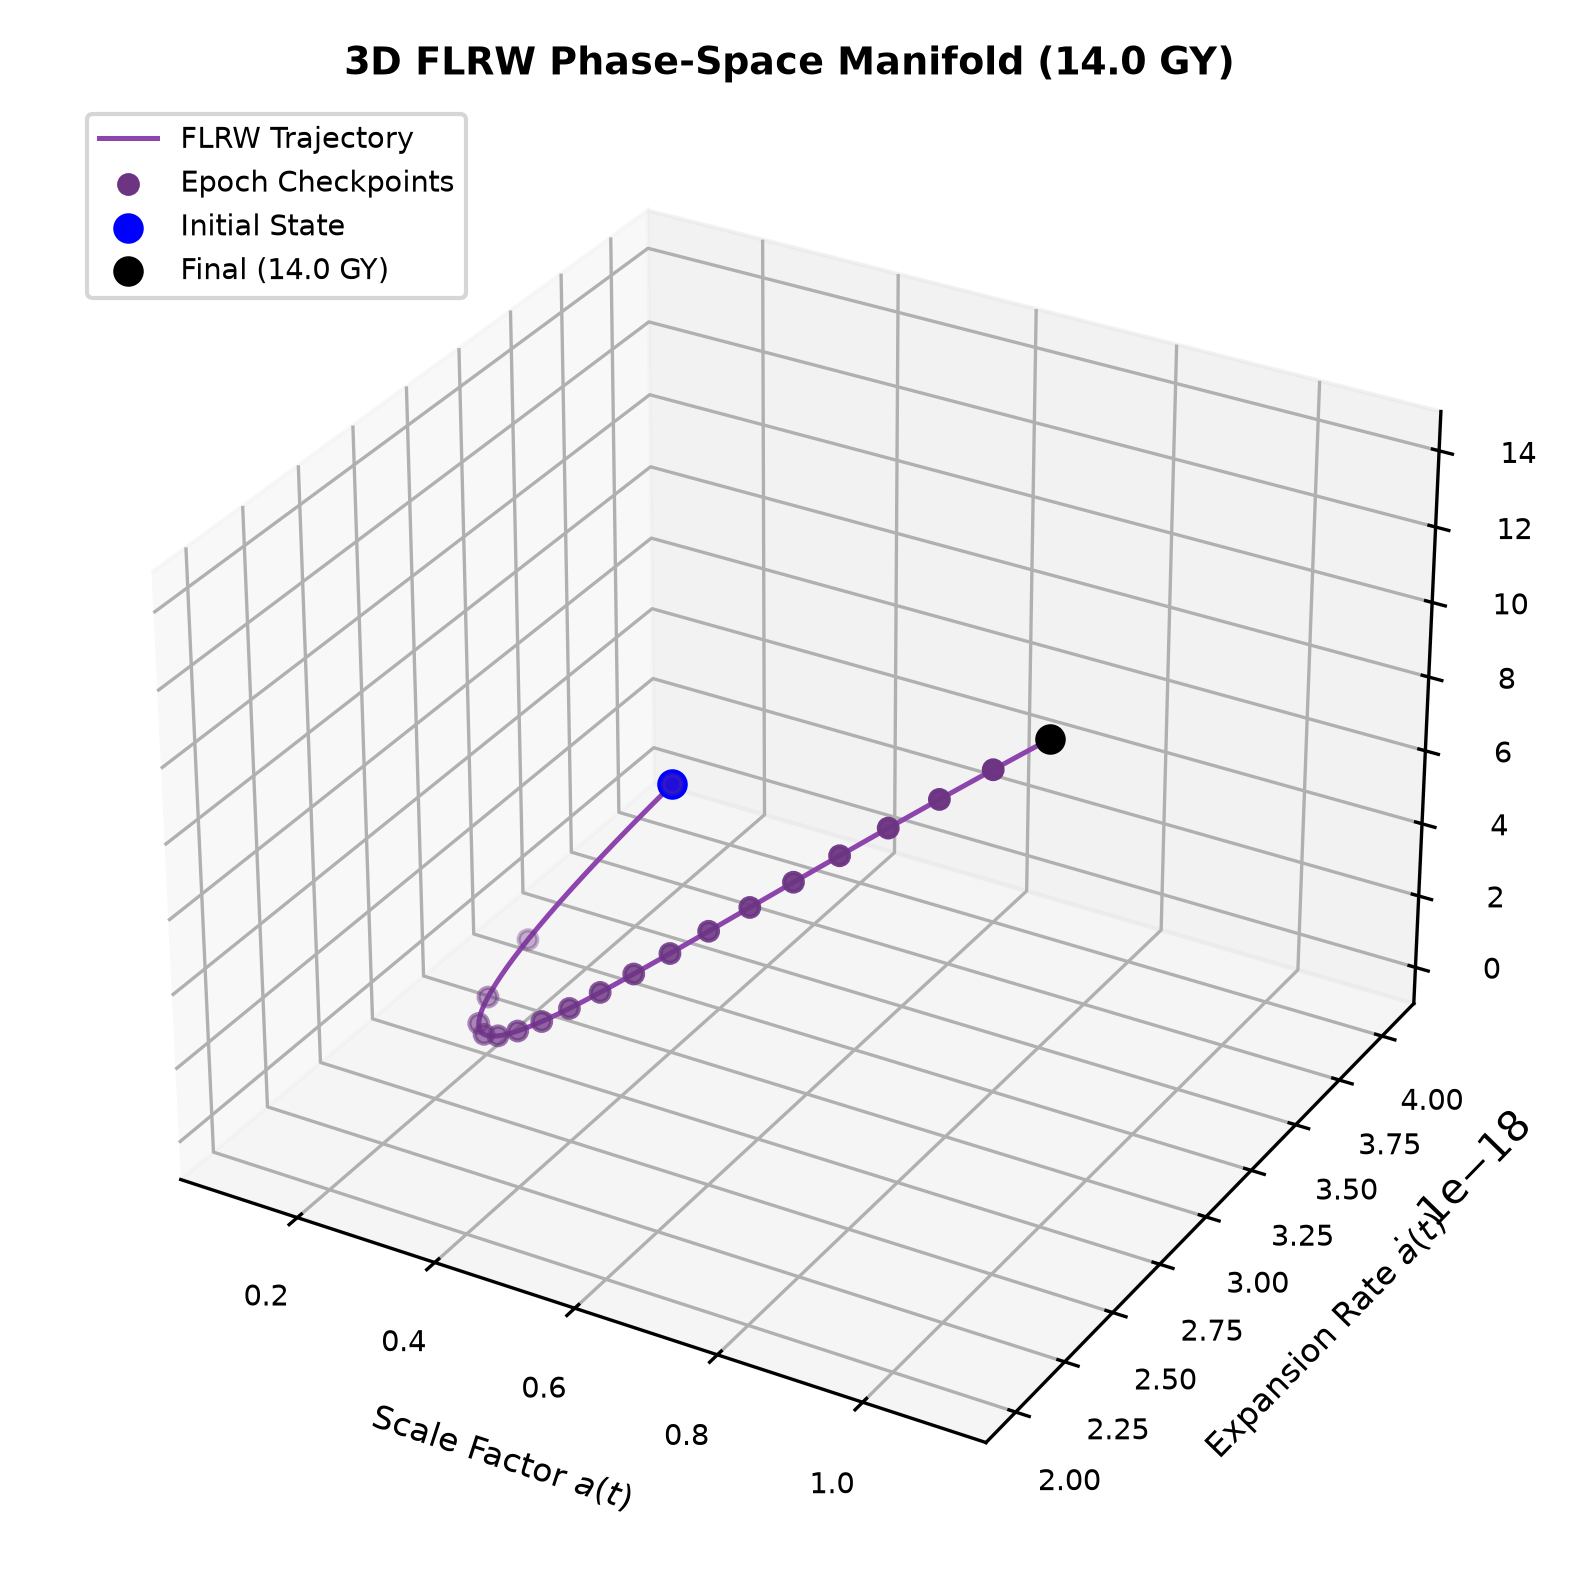
\includegraphics[width=0.5\textwidth]{contents/cosmology/the-flrw-cosmology-model-of-the-universe/phase_space_trajectory}
    \caption{Phase Space Trajectory of Scale Factor and Hubble Expansion Rate across cosmic epochs.}
    \label{fig:flrw_phase}
\end{figure}

\section{2D Evolution Plot}
\begin{figure}[h]
    \centering
    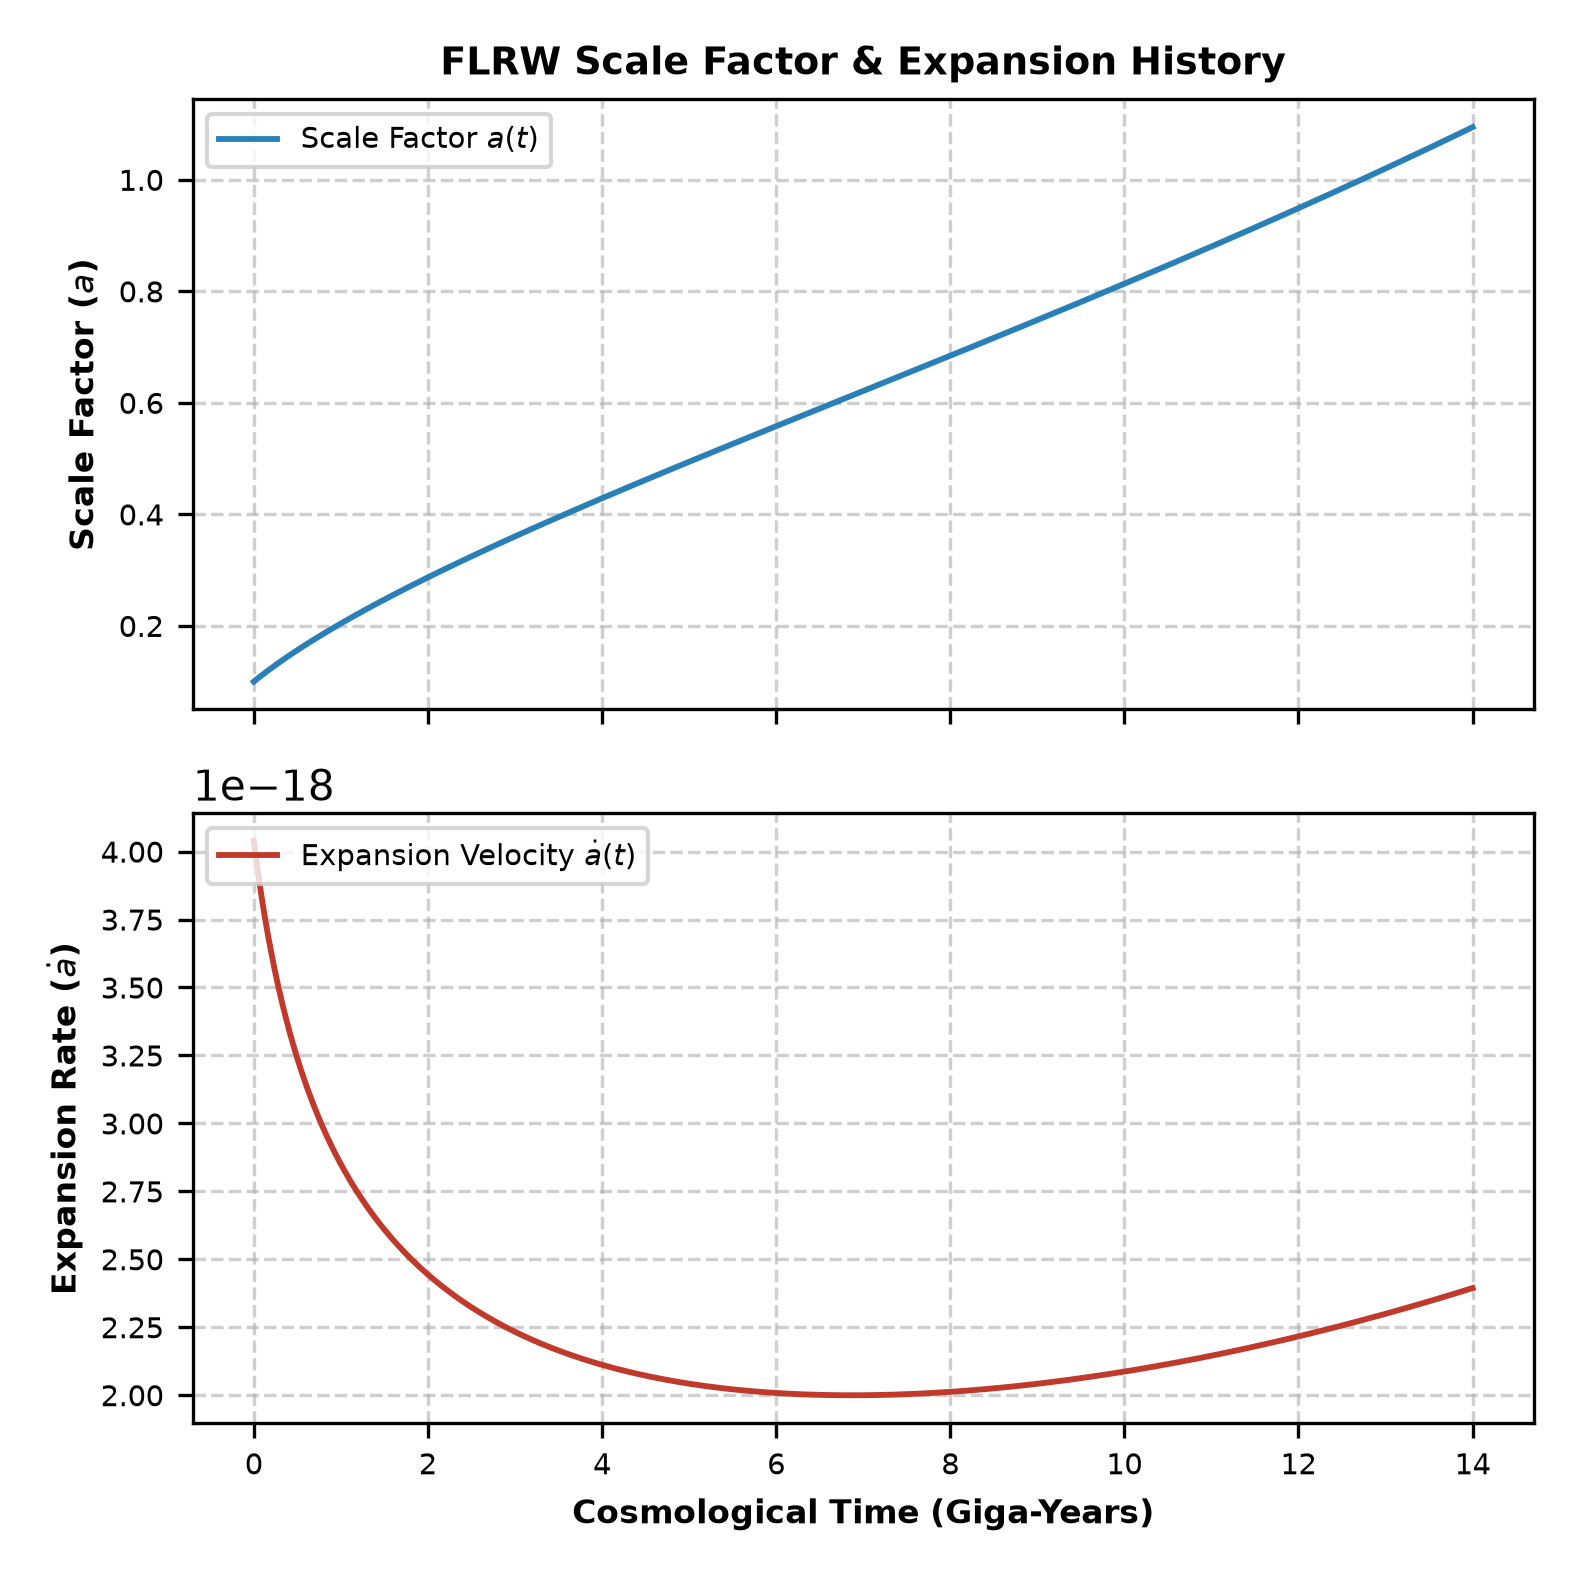
\includegraphics[width=0.5\textwidth]{contents/cosmology/the-flrw-cosmology-model-of-the-universe/system_evolution}
    \caption{2D System Evolution displaying cosmic scale factor growth and expansion rate deceleration-acceleration transition.}
    \label{fig:flrw_evolution}
\end{figure}
\clearpage
\section{Analysis of the Output}
The SDCM solver correctly tracks the transition from matter-dominated deceleration to dark-energy-driven acceleration. The scale factor evolves smoothly across cosmic time, matching standard Lambda-CDM cosmological projections without artificial energy leakage.

\section{Conclusion}
The FLRW universe model validates the SDCM framework's capacity to model relativistic cosmological expansion and cosmic metric evolution.